% !TeX spellcheck = hu_HU
% !TeX encoding = UTF-8
% !TeX program = xelatex
% TODO Change language to en_GB (recommended) or en_US for English documents
\documentclass[11pt,a4paper,oneside]{report}             % Single-side
%\documentclass[11pt,a4paper,twoside,openright]{report}  % Duplex

\input{include/packages}

%TODO Set the main variables
\newcommand{\vikszerzoVezeteknev}{Román}
\newcommand{\vikszerzoKeresztnev}{Dávid}

\newcommand{\vikkonzulensAMegszolitas}{}
\newcommand{\vikkonzulensAVezeteknev}{Tóth}
\newcommand{\vikkonzulensAKeresztnev}{Tamás}

\newcommand{\vikkonzulensBMegszolitas}{}
\newcommand{\vikkonzulensBVezeteknev}{Vörös}
\newcommand{\vikkonzulensBKeresztnev}{András}

\newcommand{\vikkonzulensCMegszolitas}{}
\newcommand{\vikkonzulensCVezeteknev}{}
\newcommand{\vikkonzulensCKeresztnev}{}

\newcommand{\vikcim}{Állapottérképek modellellenőrzése} % Cím
\newcommand{\viktanszek}{\bmemit} % Tanszék
\newcommand{\vikdoktipus}{\bsc} % Dokumentum típusa (\bsc vagy \msc)
\newcommand{\vikmunkatipusat}{Önálló labor dokumentációt} % a "hallgató nyilatkozat" részhez: szakdolgozatot vagy diplomatervet

\input{include/tdk-variables}
\newcommand{\szerzoMeta}{\vikszerzoVezeteknev{} \vikszerzoKeresztnev} % egy szerző esetén
%\newcommand{\szerzoMeta}{\vikszerzoVezeteknev{} \vikszerzoKeresztnev, \tdkszerzoB} % két szerző esetén

%TODO Language configuration -- choose one
% Beállítások magyar nyelvű dolgozathoz
%--------------------------------------------------------------------------------------
% Elnevezések
%--------------------------------------------------------------------------------------
\newcommand{\bme}{Budapesti Műszaki és Gazdaságtudományi Egyetem}
\newcommand{\vik}{Villamosmérnöki és Informatikai Kar}

\newcommand{\bmemit}{Méréstechnika és Információs Rendszerek Tanszék}

\newcommand{\keszitette}{Készítette}
\newcommand{\konzulens}{Konzulens}

\newcommand{\bsc}{Szakdolgozat}
\newcommand{\msc}{Diplomaterv}
\newcommand{\bsconlab}{BSc Önálló laboratórium}
\newcommand{\msconlabi}{MSc Önálló laboratórium 1.}
\newcommand{\msconlabii}{MSc Önálló laboratórium 2.}

\newcommand{\pelda}{Példa}
\newcommand{\definicio}{Definíció}
\newcommand{\tetel}{Tétel}

\newcommand{\bevezetes}{Bevezetés}
\newcommand{\architecture}{Arhitektúra}
\newcommand{\pojo}{A {\thetaSc} bemutatása}
\newcommand{\transzformacio}{Transzformáció}
\newcommand{\koszonetnyilvanitas}{Köszönetnyilvánítás}
\newcommand{\fuggelek}{Függelék}

% Opcionálisan átnevezhető címek
%\addto\captionsmagyar{%
%\renewcommand{\listfigurename}{Saját ábrajegyzék cím}
%\renewcommand{\listtablename}{Saját táblázatjegyzék cím}
%\renewcommand{\bibname}{Saját irodalomjegyzék név}
%}

\newcommand{\szerzo}{\vikszerzoVezeteknev{} \vikszerzoKeresztnev}
\newcommand{\vikkonzulensA}{\vikkonzulensAMegszolitas\vikkonzulensAVezeteknev{} \vikkonzulensAKeresztnev}
\newcommand{\vikkonzulensB}{\vikkonzulensBMegszolitas\vikkonzulensBVezeteknev{} \vikkonzulensBKeresztnev}
\newcommand{\vikkonzulensC}{\vikkonzulensCMegszolitas\vikkonzulensCVezeteknev{} \vikkonzulensCKeresztnev}
\newcommand{\gammaSc}{Gamma állapotgép}
\newcommand{\thetaSc}{Theta állapotgép}

\newcommand{\selectthesislanguage}{\selecthungarian}

\bibliographystyle{huplain}

\def\lstlistingname{lista}

\newcommand{\appendixnumber}{6}  % a fofejezet-szamlalo az angol ABC 6. betuje (F) lesz

% Settings for English documents
%%--------------------------------------------------------------------------------------
% Elnevezések
%--------------------------------------------------------------------------------------
\newcommand{\bme}{Budapest University of Technology and Economics}
\newcommand{\vik}{Faculty of Electrical Engineering and Informatics}

\newcommand{\bmemit}{Department of Measurement and Information Systems}

\newcommand{\keszitette}{Author}
\newcommand{\konzulens}{Advisor}

\newcommand{\bsc}{Bachelor's Thesis}
\newcommand{\msc}{Master's Thesis}
\newcommand{\bsconlab}{BSc Project Laboratory}
\newcommand{\msconlabi}{MSc Project Laboratory 1}
\newcommand{\msconlabii}{MSc Project Laboratory 2}

\newcommand{\pelda}{Example}
\newcommand{\definicio}{Definition}
\newcommand{\tetel}{Theorem}

\newcommand{\bevezetes}{Introduction}
\newcommand{\koszonetnyilvanitas}{Acknowledgements}
\newcommand{\referencia}{References}
\newcommand{\fuggelek}{Appendix}
\newcommand{\cfa}{Control Flow Automata}
\newcommand{\saai}{Static Analysis by Abstract Interpretation}

% Optional custom titles
%\addto\captionsenglish{%
%\renewcommand*{\listfigurename}{Your list of figures title}
%\renewcommand*{\listtablename}{Your list of tables title}
%\renewcommand*{\bibname}{Your bibliography title}
%}

\newcommand{\szerzo}{\vikszerzoKeresztnev{} \vikszerzoVezeteknev}
\newcommand{\vikkonzulensA}{\vikkonzulensAMegszolitas\vikkonzulensAKeresztnev{} \vikkonzulensAVezeteknev}
\newcommand{\vikkonzulensB}{\vikkonzulensBMegszolitas\vikkonzulensBKeresztnev{} \vikkonzulensBVezeteknev}
\newcommand{\vikkonzulensC}{\vikkonzulensCMegszolitas\vikkonzulensCKeresztnev{} \vikkonzulensCVezeteknev}

\newcommand{\selectthesislanguage}{\selectenglish}

\bibliographystyle{plainnat}

\newcommand{\ie}{i.e.\@\xspace}
\newcommand{\Ie}{I.e.\@\xspace}
\newcommand{\eg}{e.g.\@\xspace}
\newcommand{\Eg}{E.g.\@\xspace}
\newcommand{\etal}{et al.\@\xspace}
\newcommand{\etc}{etc.\@\xspace}
\newcommand{\vs}{vs.\@\xspace}
\newcommand{\viz}{viz.\@\xspace} % videlicet
\newcommand{\cf}{cf.\@\xspace} % confer
\newcommand{\Cf}{Cf.\@\xspace}
\newcommand{\wrt}{w.r.t.\@\xspace} % with respect to

\newcommand{\appendixnumber}{1}  % a fofejezet-szamlalo az angol ABC 1. betuje (A) lesz


\input{include/preamble}

%--------------------------------------------------------------------------------------
% Table of contents and the main text
%--------------------------------------------------------------------------------------
\begin{document}

%TODO These define guidelines -- remove these
%~~~~~~~~~~~~~~~~~~~~~~~~~~~~~~~~~~~~~~~~~~~~~~~~~~~~~~~~~~~~~~~~~~~~~~~~~~~~~~~~~~~~~~
%\include{include/guideline}
%\include{include/project}

\selectthesislanguage

%TODO Titlepage -- choose one from below
%~~~~~~~~~~~~~~~~~~~~~~~~~~~~~~~~~~~~~~~~~~~~~~~~~~~~~~~~~~~~~~~~~~~~~~~~~~~~~~~~~~~~~~
\include{include/titlepage}		   % Szakdolgozat/Diplomaterv címlap
%\include{include/titlepage-tdk}	% TDK címlap
%\include{include/titlepage-otdk}   % OTDK címlap


% Table of Contents
%~~~~~~~~~~~~~~~~~~~~~~~~~~~~~~~~~~~~~~~~~~~~~~~~~~~~~~~~~~~~~~~~~~~~~~~~~~~~~~~~~~~~~~
\tableofcontents\vfill


% Declaration and Abstract
%~~~~~~~~~~~~~~~~~~~~~~~~~~~~~~~~~~~~~~~~~~~~~~~~~~~~~~~~~~~~~~~~~~~~~~~~~~~~~~~~~~~~~~
%\include{include/declaration} %TODO Hallgatói nyilatkozat -- TDK és OTDK esetén törlendő!
%\include{content/abstract}    %TODO Összefoglaló -- TDK és OTDK esetén nem kötelező


% The main part of the thesis
%~~~~~~~~~~~~~~~~~~~~~~~~~~~~~~~~~~~~~~~~~~~~~~~~~~~~~~~~~~~~~~~~~~~~~~~~~~~~~~~~~~~~~~
\pagenumbering{arabic}

%TODO import your own content
%----------------------------------------------------------------------------
\chapter{\bevezetes}
\label{sec:intro}
%----------------------------------------------------------------------------

Todays softwares are made from millions of lines by hundreds or even thousands of programmers. According to Steve McConnell's book Code Complete on average there are 10-50 errors in 1000 lines of code. So it is inevitable that there will be a lot of mistakes during making these huge softwares. On the other hand we rely on these various parts of our lives, so if the program has bugs it causes different effects. If the outcome of this malfunction dangers great fortunes os human health or even lives than we say it is a safety critical system. We want to make sure that these systems are fault proof. Static analysis is a method to analyze the software without actually executing it, detecting possible vulnerable part of the source code. Some problems such as simple coding errors are easy to find, however we can detect other, more complicated vulnerabilities like possible zero division or other logical errors. However checking the whole software can be impossible within a reasonable time. In this case abstracting can simplify the problem, and make it possible to analyze certain behaviors of the software. 

Static Analysis by Abstract Interpretation (SAAI) was introduced by Cousot in \hyperref[sec:ref]{[2]}. An easy to understand description is available at \hyperref[sec:ref]{[1]}. Able to analyze certain behaviors of the software, by making an abstraction which focuses on this behavior so it is much simpler than the whole software, but the required conditions can still be tested. There are plenty of abstraction methods such as sign or interval abstraction. 





%----------------------------------------------------------------------------
\chapter{\architecture}
\label{sec:archiutecture}

Ebben a fejezetben megmutatom milyen már működő keretrendszereket használtam, illetve próbáltam hozzájárulni fejlesztésükhöz a féléves munkám során

%----------------------------------------------------------------------------
\section{Gamma keretrendszer}
%----------------------------------------------------------------------------
A félév során megpróbáltam már meglévő keretrendszerekbe beledolgozni. Ilyen keretrendszer a Gamma\footnote{A Gamma hivatalos oldala: \url{https://inf.mit.bme.hu/node/6028}}, ami a tanszéken fejlesztett rendszer és összetett állapotgépek analízisét teszi lehetővé számos eszköz segítségével.

Az Uppaal modell ellenőrző\footnote{Az Uppaal weboldala: \url{http://www.uppaal.org/}} például lehetővé teszi a {\gammaSc} modellellenőrzését. Viszont ez az eszköz nem tudja kezelni az összetett állapotgépeket, ezért át kell alakítani a {\gammaSc}et, hogy ne legyenek már benne összetett állapotok, ekkor viszont információt veszítünk\footnote{Magyarázat \hyperref[infovesztes]{Az összetett állapotgépeknél}} és az analízis jelentősen lassabb lehet. Van igény tehát olyan modellellenőrzésre a Gamma keretrendszeren belül, ami kihasználja az összetettséget.

A {\gammaSc}ek EMF\footnote{Eclipse Modelling Framework \url{https://www.eclipse.org/modeling/emf/}} és XTEXT\footnote{\url{https://www.eclipse.org/Xtext/}} technológiát használnak, ami nehezebbé teszi a modell architektúra tetszőleges kialakítását, ezért a félév során egy új ezektől a technológiáktól nem függő állapotgép Pojo-t csináltam amit, majd a következő fejezetben fogok bemutatni.

Még egy hasznos funkciója a Gammának, hogy lehet vele Yakindu\footnote{Egy nagyon elterjedt állapotgép szerkesztő eszköz, weboldala: \url{https://www.itemis.com/en/yakindu/state-machine/}}-ban szerkesztett állapotgépeket {\gammaSc}pé alakítani.


%----------------------------------------------------------------------------
\section{Theta keretrendszer}
%---------------------------------------------------------------------------- 

A Theta\footnote{hivatalos weboldala: \url{https://inf.mit.bme.hu/en/theta}} szintén a tanszéken fejlesztett eszköz, (ami egyéb dolgok mellett) interfészt nyújt több SMT Solverhez, megvalósít különböző absztrakciós módszereket. Ezek a funkciók nagyon hasznosak lehetnek az állapotgépek modellellenőrzéséhez.

Nem meglepő tehát, hogy a már említett Pojo-t ebbe a keretrendszerbe szeretnénk beépíteni. Ezt a Pojo-t innentől tehát {\thetaSc}-nek fogom nevezni. 
%----------------------------------------------------------------------------
\chapter{\pojo}
\label{sec:pojochapter}

Ebben a fajezetben bemutatom a {\thetaSc} reprezentációt. Mivel egy már korábban mások által elkezdett projektet fejeztem be külön kitérek arra is, hogy mely részek a saját fejlesztésem részei.
%----------------------------------------------------------------------------
\section{Az állapotgép}
%----------------------------------------------------------------------------
Az állapotgép egy széles körben használt modellezési módszer. A modellezni kívánt rendszerünket több egymástól jól elkülöníthető állapotokra bontjuk, ez lesz a rendszer állapota. Elvégezhetünk különféle feladatokat, akkor ha belépünk, vagy akkor ha kilépünk az adott állapotból.

\begin{figure} [!ht]
\centering
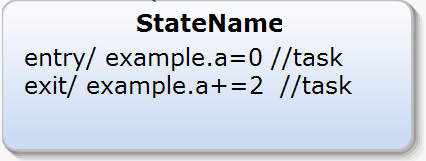
\includegraphics[width=60mm, keepaspectratio]{figures/state.png}
\caption{\label{fig:state}Egy állapot Yakinduban.}
\end{figure}

A rendszer természetesen működés közben változik, másik állapotba kerül. Az állapotváltást a tranzíciók segítségével írjuk le. Ezeket mindig valamilyen esemény váltja ki, lehet egy felhasználói esemény, vagy egy időzített esemény. Őrfeltételt is adhatunk \verb+[]+-en belül ilyenkor csak akkor lépünk át a másik állapotba, ha ez a feltétel teljesül. A \verb+/+ után pedig újabb parancsokat hajthatunk végre

\begin{figure} [!ht]
 	\centering
 	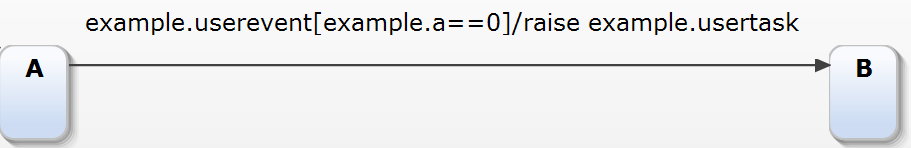
\includegraphics[width=150mm, keepaspectratio]{figures/transition.png}
 	\caption{\label{fig:transition}Egy tranzíció Yakinduban.}
\end{figure}

Előfordulhat az is, hogy több állapotot valamilyen közös tulajdonságuk szerint szeretnénk csoportosítani. Ilyenkor jók az összetett állapotok.\label{infovesztes} Ezt az információt veszítjük tehát el, ha "kilapítjuk"\footnote{Több állapot felvételével helyettesítjük az összetett állapotokat} az állapotgépet.

Itt kell bevezetni a régió fogalmát. Minden állapot egy régióban van, és minden régióban egyszerre csak egy állapot írhatja le a rendszerünket. Az összetett állapotok tehát tartalmaznak legalább egy régiót.

A régión belül van egy úgynevezett pszeudó állapot, ami kijelöli, hogy egy régióba lépés esetén melyik állapotba lépjünk. Három fajtája van a history, deephistory és a sima kezdő állapot. A sima mindig ugyanarra az állapotra mutat, a history megjegyzi, hogy kilépéskor melyik volt aktív és oda léptet vissza. A deephistory még ennél is többet jegyez meg, ha a kilépéskori aktív állapot, egy összetett állapot, akkor az azon belüli aktív állapotokat is megjegyzi.

\begin{figure} [!ht]
	\centering
	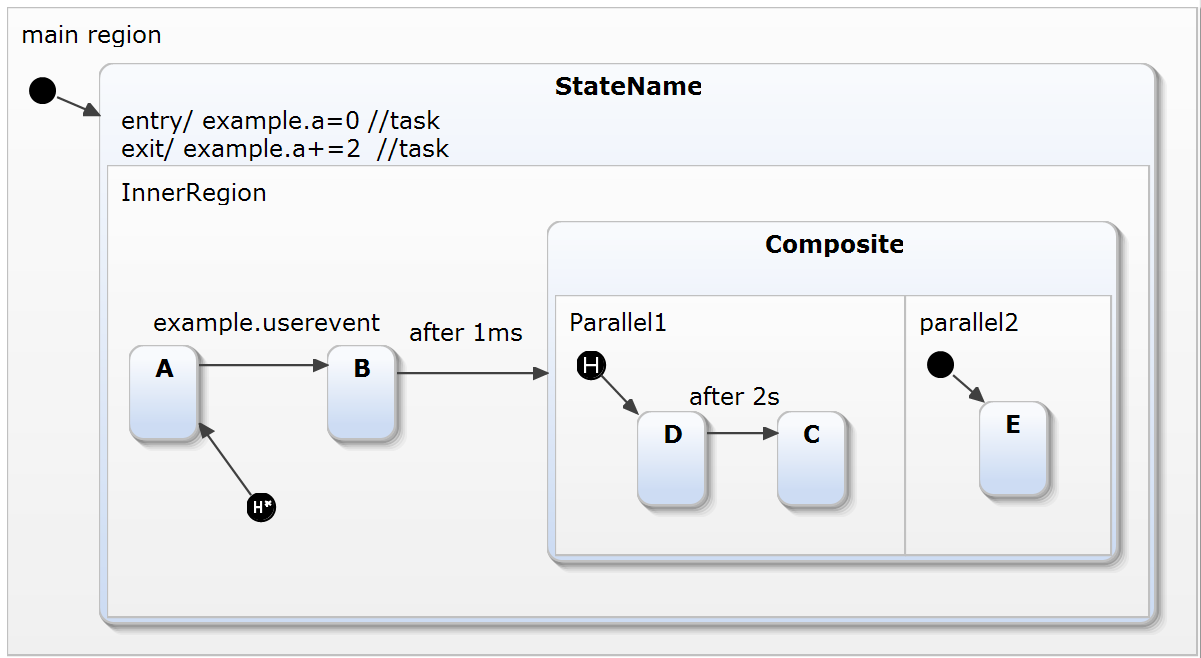
\includegraphics[width=150mm, keepaspectratio]{figures/statechart.png}
	\caption{\label{fig:statechart}Egy összetett állapotgép Yakinduban.}
\end{figure}


%----------------------------------------------------------------------------
\section{A {\thetaSc}}
\label{sec:thetaleiras}
%----------------------------------------------------------------------------

Az állapotgép reprezentáció Java-ban készült el. Az egyes osztályok megfeleltethetők az előző fejezetben leírt állapotgép elemekkel. Mindegyik osztálynak vannak a tárolt elemeihez getter/setter, a tárolóikhoz pedig add függvényei. Illetve néhány segédfüggvény, ami segít majd az analízis közben. A projekt már korábbi munkák folytatásaként jött létre. Az én hozzájárulásom a pszeudó állapotok implementálása, az időzített események kezelése és néhány segéd függvény, illetve apróbb javítások.


\begin{lstlisting}[language=java,breaklines=true]
interface Sc {}
\end{lstlisting}

Az állapotgépet reprezentáló interfész. Ez tárolja a gyökér régiót. Van neve, tárolja az összes tranzíciót az állapotgépben. Tárolja a változó deklarációkat egy a Thetában értelmezett osztályban (VarDecl). 

Az egyetlen megvalósító osztály a \verb+MutableSc+ minden tárolója hashSet-ben van megvalósítva

\begin{lstlisting}[language=java,breaklines=true]
interface Region {}
\end{lstlisting}

Van neve, tárolja az állapotait (State), ezek lekérdezhetőek és pontosan egy pszeudó állapota (PseudoState) van. Lehet szülő állapota; az állapot ami közvetlen őt tartalmazza. Továbbá van egy Boolean attribútuma, ami azt jelzi, hogy RootRegion-e a régió azaz nincs neki szülőállapota. Ellenőrizhető, hogy szabályos-e a régió: Minden tartalmazás igaz fordított irányban (vagyis az elem szülő eleme a régió)

Az egyetlen megvalósító osztály a \verb+MutableRegion+ egy hashSet-ben tárolja az állapotait

\begin{lstlisting}[language=java,breaklines=true]
interface State {}
\end{lstlisting}

Van neve és tárolja a régióit (Region) ez lehet egy üres lista. Kötelezően van szülő régiója. Van két akciója (Action), egy a kimeneti, egy a bemeneti akcióknak. Van két tranzíció tárolója, tárolja ugyanis a beérkező tranzíciókat és a kimenőket is.

Az egyetlen megvalósító osztály a \verb+MutableState+ minden tárolója hashSet-ben van megvalósítva

\begin{lstlisting}[language=java,breaklines=true]
interface Transition {}
\end{lstlisting}

A tranzíciót reprezentáló interfész. Tárolja a forrás állapotát (honnan indul ki) és a cél állapotát (hova érkezünk). Továbbá van egy kiváltó (trigger) eseménye (Event). Lehet őrfeltétele, ami a Thetában is használt Expr<Type> osztály. Van egy akciója (Action)

Az egyetlen megvalósító osztály a \verb+MutableTransition+

\begin{lstlisting}[language=java,breaklines=true]
interface PseudoState {}
\end{lstlisting}

Van neve, tárolja azt az egy állapotot ami a régiójába lépéskor az aktuális állapot lesz. Kötelezően kell legyen egy szülő régiója (Region).

Három megvalósító osztály a \verb+MutableInitState+ a sima kezdő ~ a \verb+MutableHistorytate+ a history~ a \verb+MutableDeepHistoryState+ pedig a deephistory pszeudó állapothoz

\begin{lstlisting}[language=java,breaklines=true]
interface Action {}
\end{lstlisting}

Interfész az akcióknak. Visitor mintát követi. Négy különböző osztály van. 

Az \verb+AssignmentAction+ egy egyszerű változó értékadást reprezentál, van tehát egy változója (VarDecl) és egy kifejezése (Expr).

A \verb+SignalAction+ egy esemény (Event) jelzést reprezentál. Ennek megfelelően tárol egy eseményt (csak egyet)

Az \verb+EmptyAction+ azért van, hogy ne null-okat tároljunk ha egy tranzíciónak, vagy állapotnak nincs akciója

A \verb+SequenceAction+ Több akciót (Action) tárol

\begin{lstlisting}[language=java,breaklines=true]
interface Event {}
\end{lstlisting}

Az eseményeket reprezentáló interfész alapvetően, csak egy neve van.

Két megvalósító osztály van az \verb+EventImpl+ a user eseményekhez, a \verb+TimeEventImpl+ pedig az időzített eseményeknek a \hyperref[fig:statechart]{3.3-as ábrán} is látható after 2s is egy ilyen esemény. Tárolja a nevén kívül azt, hogy mennyi az időzítés (milliszekundumban).


%----------------------------------------------------------------------------
\section{Sorosítás}
%----------------------------------------------------------------------------

Amikor egy adott modellen akarunk végezni analízist, valószínűleg nem csak egyszer tesszük ezt meg, hanem többször is. Nem lenne túl hatékony, ha mindig újra kéne építeni az állapotgépet, erre van a sorosítás, vagy szerializáció, ami lehetővé teszi az állapotgépek gyors beolvasását, illetve akár néhány módosítás utáni kiírását.

A séma Lisp-szerű szintaxist követ. A \hyperref[sec:thetaleiras]{fent} említett elemek sorosítva a következőképp néznek ki:

\begin{lstlisting}[language=java,breaklines=true]
(statechart nameOfStateChart
	(var varName varType)
	(var var2 type)
	(event Esemény)
	(region regionName
		(state stateName
			(entry assign varName value)
			(exit assign var2 value))
		(state compositeState
			(region innerRegion
				(state inState)
				(state stateA))
				(init inState))
		(history stateName))
	(transition stateName compositeState
		(trigger Esemény)
		(guard varName>2)
		(effect 
			(sequence
					(assign varName value)
					(signal Esemény))))
\end{lstlisting}

Azt érdemes megemlíteni, hogy egy-egy elemet előbb deklarálunk, például (var varName varType) és utána már elég a nevével hivatkozni rá. Például (assign varName value)

\begin{figure} [!ht]
	\centering
	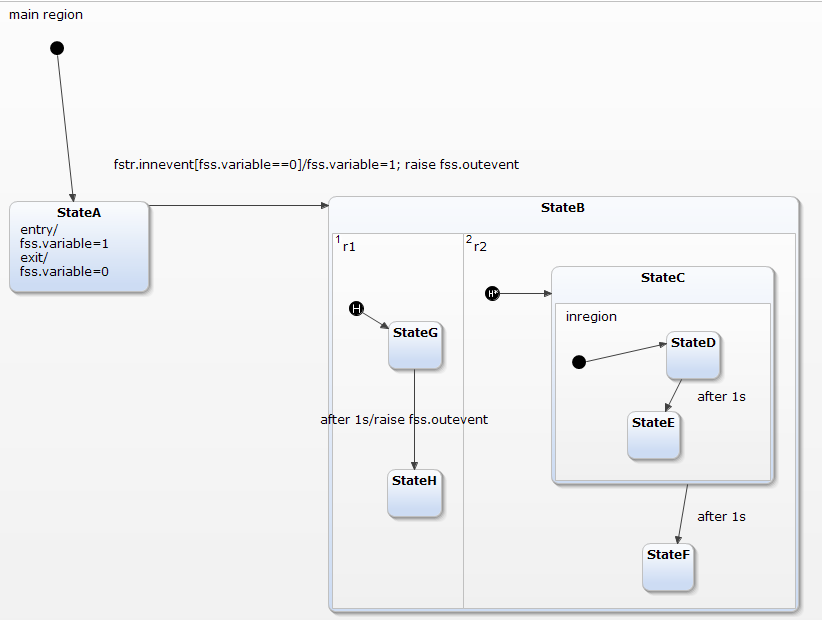
\includegraphics[width=150mm, keepaspectratio]{figures/serializeexample.png}
	\caption{\label{fig:serializeexample}példa állapotgép a szerializációhoz}
\end{figure}

\begin{figure} [!ht]
\centering
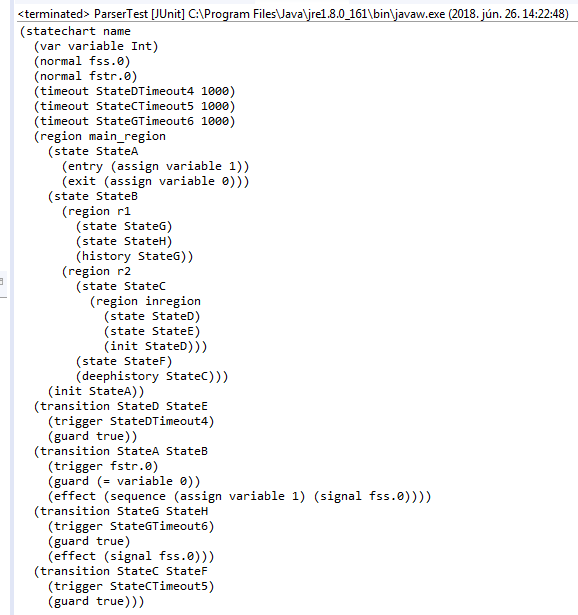
\includegraphics[width=150mm, keepaspectratio]{figures/serializeresult.png}
\caption{\label{fig:serializeresult}a \hyperref[fig:serializeexample]{fenti} állapotgép sorosítva}
\end{figure}


%----------------------------------------------------------------------------
\chapter{\transzformacio}
\label{sec:transzformacio}

A Gamma keretrendszert is szeretnénk összekötni az \hyperref[sec:thetaleiras]{előző} fejezetben bemutatott {\thetaSc}pel. Ezért írtam egy segéd osztályt, ami képes a beolvasott EMF-es {\gammaSc}et átalakítani {\thetaSc}pé.
%----------------------------------------------------------------------------
\section{{\gammaSc}}
%----------------------------------------------------------------------------
Már korábban említettem az \hyperref[sec:archiutecture]{Architektúra} fejezetben, hogy a {\gammaSc} egy EMF alapú állapotgép reprezentáció. Így a sémája nem sokban különbözik az \hyperref[sec:thetaleiras]{előző} fejezetben leírt {\thetaSc}től. Ez megkönnyíti a transzformáció folyamatát. Az erre a célra írt segédosztályokat mutatom be a következő részekben


%----------------------------------------------------------------------------
\section{GammaSctoThetaSCConverter}
%----------------------------------------------------------------------------

Ez az osztály egy statikus \verb+convert()+ függvény meghívásával transzformál

\begin{lstlisting}[language=java ,breaklines=true]
public static MutableSc Convert(final StatechartDefinition gammaSC, final String name) 
\end{lstlisting}

Látható, hogy bemenetként egy beolvasott EMF gyökér elemet várunk (ez a {\gammaSc}et reprezentáló StatechartDefinition osztály) a name pedig a {\thetaSc} neve lesz.

Először beolvassuk a változókat, ezekkel létrehozok egy ExpressionConverter-t amit a következő szekcióban mutatok be. Utána beolvassuk a gyökér régiót ami az addRegiontoThetaSC() rekurzív függvény meghívásával történik utána a tranzíciókat adom az állapotgéphez (frissítve a már korábban létrehozott állapotokat)

\begin{lstlisting}[language=java ,breaklines=true]
private static void addRegiontoThetaSC(final Region reg, final MutableRegion r) 
\end{lstlisting}

Ez a függvény rekurzív, abból a szempontból, hogy ha egy régión belül van egy másik régió akkor meghívja önmagát. Minden elemhez van egy ehhez hasonló függvény, aminek a bemenete, egy gammás elem és egy annak megfelelő Thetás elem, és a transzformátor a gammás elemben lévő belső elemeket létrehozza és berakja a Thetás elembe. Ez így megy addig amíg az adott elemekben vannak újabb elemek.

%----------------------------------------------------------------------------
\section{ExpressionConverter}
%----------------------------------------------------------------------------

A legnagyobb nehézség az akciókban illetve őrfeltételekben használt kifejezések megfelelő átkonvertálása, ehhez használom a ExpressionConverter segéd osztályt. A Thetában van erre egy segítség a DispachTable. Ennek a segítségével könnyen és átláthatóan össze lehet kötni a különböző gammás Expression-öket a Thetás Expr<> osztályokkal

%----------------------------------------------------------------------------
\chapter{Állapotgép konfiguráció}
\label{sec:stateconfig}
%----------------------------------------------------------------------------
\section{Aktív állapot}
%----------------------------------------------------------------------------
Az állapotgép a rendszerünk összes lehetséges állapotát mutatja. Analízis közben azonban fontos hogy azt is tudjuk nézni, hogy mik az aktív állapotok, azaz melyek írják le a rendszerünk pillanatnyi helyzetét.

Az aktív állapotoknak van több szabálya.
\begin{itemize}
	\item Egy régión belül, pontosan egy aktív állapot lehet (közvetlen gyerekekre nézve)
	\item Egy aktív állapot összes szülő állapota is aktív
	\item Minden régióban van aktív állapot
\end{itemize}

%----------------------------------------------------------------------------
\section{A megvalósító osztály}
%----------------------------------------------------------------------------

A StateConfiguration osztályban valósítom meg. Egy ilyen példány tartalmazza az állapotgép reprezentációt (Sc) továbbá egy listát az épp aktuális állapotokról és -egy később igen hasznosnak bizonyuló segítség- tároljuk, hogy az adott konfiguráció mely tranzíciók elsütésével érhető el a kiindulási állapotból, illetve hogy eközben milyen akciók lettek végrehajtva. Oly módon, hogy minden egyes tranzícióhoz ebben a listában két akció tartozik, egy azokhoz az akciókhoz, amik a tranzíció őrfeltétel ellenőrzés előtt hajtódnak végre, egy pedig azokhoz amik utána.

\begin{lstlisting}[language=bash,morekeywords={sudo,apt\-get},alsoletter={-},breaklines=true]
public static StateConfiguration create(final Sc sc)
\end{lstlisting}

Létrehozható egy {\thetaSc}ből.

\begin{lstlisting}[language=bash,morekeywords={sudo,apt\-get},alsoletter={-},breaklines=true]
public void init()
\end{lstlisting}

Aktiválja az állapotgépet, azaz mindenhol a kezdő állapot szerint kijelöli az aktív állapotokat

\begin{lstlisting}[language=bash,morekeywords={sudo,apt\-get},alsoletter={-},breaklines=true]
	public Collection<Transition> getFireableTransitions()
\end{lstlisting}

Visszaad egy listát az összes olyan tranzícióról, ami tüzelhető az adott konfigurációban. Vagyis a tranzíció forrásállapota aktív.

\begin{lstlisting}[language=bash,morekeywords={sudo,apt\-get},alsoletter={-},breaklines=true]
public StateConfiguration fire(final Transition tr)
\end{lstlisting}

Visszaad egy új állapotgép konfigurációt, ami a paraméterben megadott tranzíció elsütése után kialakul. Saját magát nem változtatja!


%----------------------------------------------------------------------------
\chapter{Korlátos modell ellenőrző}
\label{sec:bmc}
%----------------------------------------------------------------------------
\section{Modell ellenőrzés}
%----------------------------------------------------------------------------
A \hyperref[sec:intro]{bevezetőben} már elmondtam miért fontos a modellellenőrzés, most inkább arról beszélek, hogy ez mit jelent az állapotgépek esetén. A \hyperref[fig:mcheck]{6. 1-es ábrán} látható a működés elve. A modellellenőrző tehát egy modell reprezentációt, és egy tulajdonságot kap bemenetként. És megadja, hogy teljesül-e az adott tulajdonság, vagy nem. Ilyenkor még egy példát is ad arra, amikor nem teljesül, amivel könnyen ellenőrizhetjük, hogy igaz volt-e. A másik esetben viszont, ha nem talál ellenpéldát akkor azt bebizonyítani, hogy valóban nincs, csak úgy lehet, ha a modellellenőrző működés közben bizonyítottan megtalál minden ellenpéldát. Ezt sokszor csak bizonyos korlátok mellett lehet biztosítani.

A tulajdonság, általában egy elérhetőségi vizsgálatot jelent\footnote{Elérhető-e egy állapot a kezdeti állapotkonfigurációból, úgy, hogy minden tranzíció elsütése érvényes, azaz teljesül az őrfeltétel}. A BMC\footnote{Bounded Model Checker, a korlátos modell ellenőrző rövid neve}-nél sincs ez másképp, ilyenkor az ellenpélda egy útvonal az elérni kívánt állapothoz\footnote{Mely tranzíciókat kell elsütni, milyen sorrendben}. Mivel azt szeretjük, ha a hibás esetekben van ellenpélda ez az állapot egy hibaállapot, ami a rendszer nem megfelelő működését jelzi.

A BMC a helyes működést, azaz hogy egy állapot biztosan nem érhető el nem tudja bizonyítani, mert végtelen ideig is tarthatna a futás ideje. Ezért inkább megfogalmaz egy korlátot: maximum K lépésből elérhető-e az adott állapot

\begin{figure}[!ht]
	\centering
	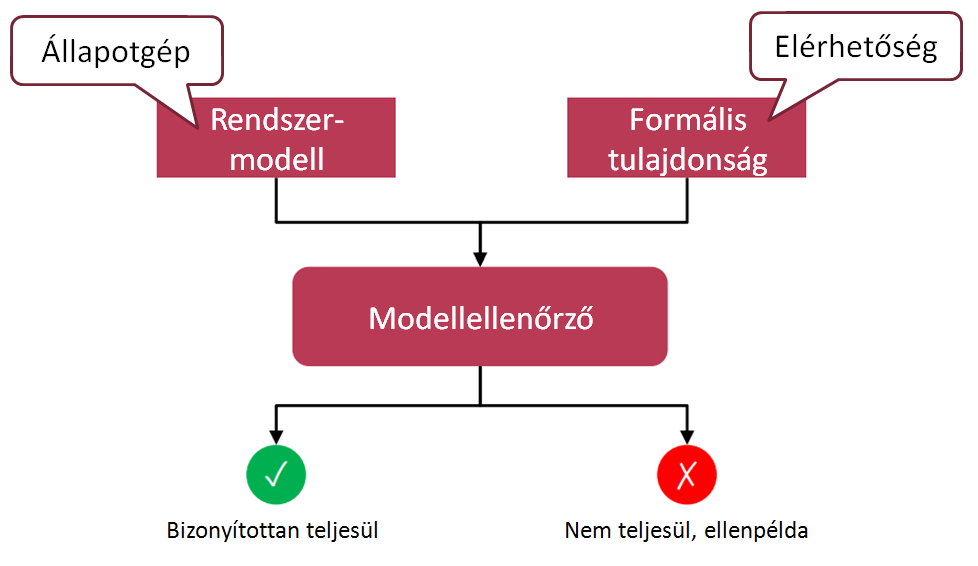
\includegraphics[width=74mm, keepaspectratio]{figures/altmc.png}\hspace{0cm}
	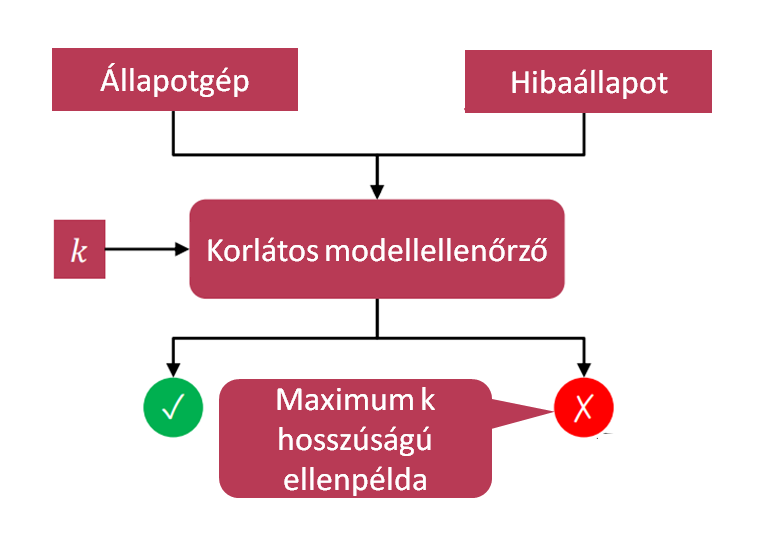
\includegraphics[width=74mm, keepaspectratio]{figures/bmc.png}
	\caption{Az általános ~ (balra) és a korlátos modellellenőrző (jobbra) működési elve}
	\label{fig:mcheck}
\end{figure}


%----------------------------------------------------------------------------
\section{A BMC menete}
%----------------------------------------------------------------------------
A korlátos modellellenőrző működése a \hyperref[fig:bmcfolyamat]{6.2-es ábrán} látható. A keresés egy szélességi gráf
bejárás az állapotkonfigurációkon ahol a k korlát mélységig megyünk. A hiba állapot olyan állapotgép konfigurációt jelent, ahol a hibaállapot aktív.

\begin{figure}[!ht]
	\centering
	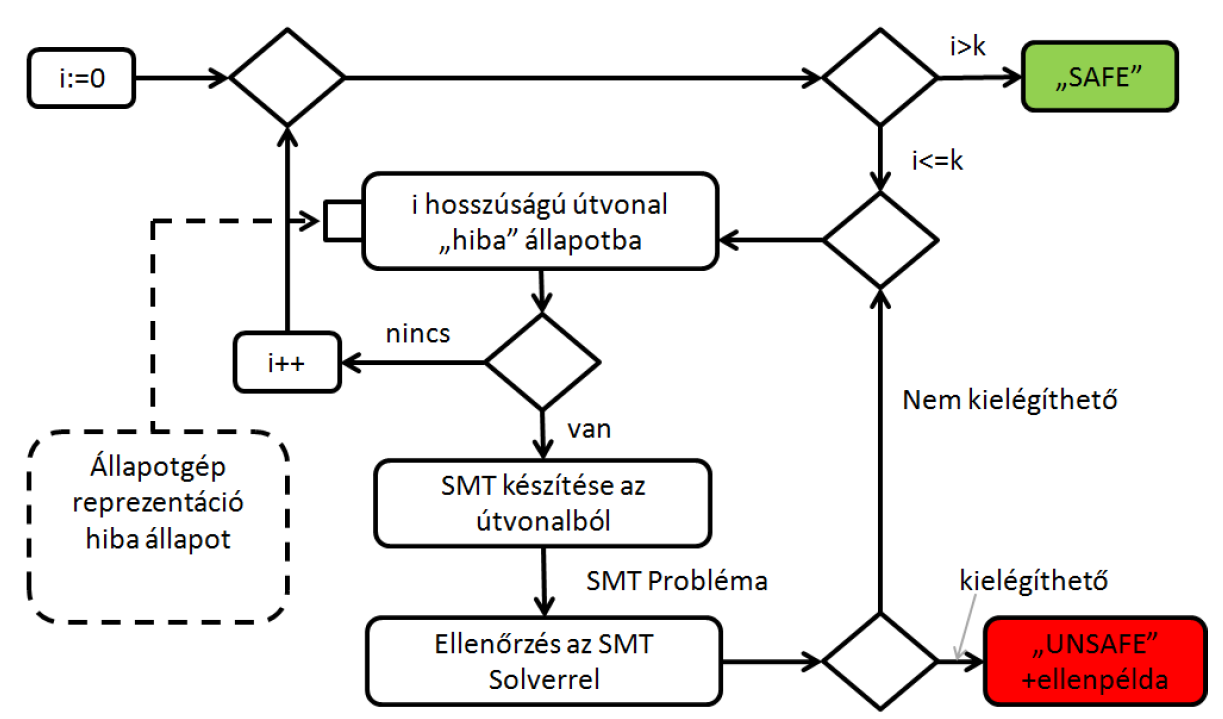
\includegraphics[width=150mm, keepaspectratio]{figures/bmcfolyamatmodell.png}
	\caption{A korlátos modellellenőrző folyamat modellje}
	\label{fig:bmcfolyamat}
\end{figure}

%----------------------------------------------------------------------------
\section{Az útvonal}
%----------------------------------------------------------------------------
A \verb+Path+ osztályt használom ennek a leírására. Tárolom az összes állapotgép konfigurációt az kiinduló állástól kezdve, és az útvonal során elsütött tranzíciókat.


\begin{lstlisting}[language=java,breaklines=true]
public boolean checkpath()
\end{lstlisting}

Azt ellenőrzi, hogy az útvonal helyes-e azaz minden egyes konfigurációból valóban jó konfigurációba léptünk és az elsütött tranzíció elsüthető volt (a forrásállapota aktív volt)

\begin{lstlisting}[language=java,breaklines=true]
public StateConfiguration getResultConfiguration()
\end{lstlisting}

Az útvonal végigfutása utáni állapotkonfigurációt adja vissza


%----------------------------------------------------------------------------
\section{SMT Solver}
%----------------------------------------------------------------------------
Az SMT solver egy olyan eszköz, ami több aritmetikai kifejezést kapva, megtudja mondani, hogy ezek teljesülhetnek-e egyszerre. Ha igen akkor ad egy példa értéket az összes benne szereplő változóra, hogy azok kielégítsék mindegyik aritmetikai kifejezést.

Ezek most nekünk azért kellenek, mert az útvonalakon, a tranzíciókon lévő őrfeltételek is egy ilyen aritmetikai kifejezéshalmazt képeznek. 

A Theta projektben van egy interfész a Z3 solveréhez, ezt használtam.

Az \verb+SMTBuilder+ segéd osztályban csinálok az útvonalak segítségével SMT problémát, amit át tudok adni a solvernek.

\begin{lstlisting}[language=java,breaklines=true]
public SMTBuilder(final Path p) {
\end{lstlisting}
A segéd osztály egyszerűen létrehozható az útvonal alapján.


\begin{lstlisting}[language=java,breaklines=true]
public Collection<Expr<BoolType>> unfold()
\end{lstlisting}

Ezzel a függvénnyel hozzuk létre azt a listát, amit közvetlen átadhatunk a solvernek. 

Elsőre egyszerűnek tűnik, hiszen a tranzíciók, már ezt a formátumot használják az őrfeltételek tárolásához, de figyelemmel kell kísérni azt is, hogy az akciók során változhatnak a változó értékei -akár többször is-. Ennek a problémának a megoldásához van egy eszköz a Theta projekten belül (\verb+PathUtils+), ami pont ennek a "változó frissítésnek" ad implementációt. Itt válik hasznossá, hogy az \hyperref[sec:stateconfig]{állapotgép konfigurációkban tároljuk az összes akciót, ami a kezdeti állapothoz képest történt}.

%----------------------------------------------------------------------------
\section{BoundedChecker}
%----------------------------------------------------------------------------
Maga az ellenőrző osztály a \verb+BoundedChecker+.

\begin{lstlisting}[language=java,breaklines=true]
public BoundedChecker(final Sc chart, final int K, final State errorState)
\end{lstlisting}

Bemenetként egy állapotgépet várunk, amin végezzük az ellenőrzést. Bekérünk egy K korlátot, ami megadja a maximum lépés számot, és persze maga a hiba állapotot is kell.

\begin{lstlisting}[language=java,breaklines=true]
	public SafetyStatus check()
\end{lstlisting}

Ezzel a függvénnyel lehet futtatni az ellenőrzést, egy \verb+SafetyStatus+ al tér vissza amiből kiolvasható, hogy biztonságos-e, ha nem, akkor az ellenpéldát is ki lehet olvasni. Meghívja az \verb+algorithm+ függvényt

\begin{lstlisting}[language=java,breaklines=true]
public SafetyStatus algorithm(final Collection<Path> paths, final int deep) 
\end{lstlisting}

Egy rekurzív függvény ami, minden egyes lépésben növeli a mélységet (deep) és, minden útvonalból, (ami nem bukott már meg) létrehozza az összes lehetséges új útvonalakat. Ehhez elég az útvonal utolsó konfigurációján minden elsüthető tranzíciót elsütni.

Így biztosítjuk azt, hogy az összes lehetséges útvonalat megnézzük, aminek a hossza az inicializáláskor megadott maximumnál nem nagyobb. Tehát, ha nem találunk ellenpéldát akkor biztosan állíthatjuk, hogy nincs is.

A bizonyítás azért nem ennyire egyszerű, mert ugyan kipróbálunk minden lehetőséget, előfordulhat, hogy egy jó ellenpéldát nem fogadunk el, ez persze úgy lehet, ha például, rosszul építjük meg az SMT problémát és azt kapjuk, jogtalanul, hogy az útvonal nem teljesíthető.

További információ a \hyperref[sec:verifikacio]{verifikációs} résznél



%----------------------------------------------------------------------------
\chapter{Verification}
\label{sec:verifikacio}

%----------------------------------------------------------------------------
\section{The Abstraction library usage}
%----------------------------------------------------------------------------
Implementing an abstraction type:

Run reachability analysis:

%----------------------------------------------------------------------------
\section{Performance measurements}
%----------------------------------------------------------------------------


%----------------------------------------------------------------------------
\section{Tests on the implemented abstraction algorithms}
%----------------------------------------------------------------------------



%\include{content/latex-tools}
%\include{content/thesis-format}
%\include{content/template-usage}


% Acknowledgements
%~~~~~~~~~~~~~~~~~~~~~~~~~~~~~~~~~~~~~~~~~~~~~~~~~~~~~~~~~~~~~~~~~~~~~~~~~~~~~~~~~~~~~~
%\include{content/acknowledgement}


% List of Figures, Tables
%~~~~~~~~~~~~~~~~~~~~~~~~~~~~~~~~~~~~~~~~~~~~~~~~~~~~~~~~~~~~~~~~~~~~~~~~~~~~~~~~~~~~~~
%\listoffigures\addcontentsline{toc}{chapter}{\listfigurename}
%\listoftables\addcontentsline{toc}{chapter}{\listtablename}


% Bibliography
%~~~~~~~~~~~~~~~~~~~~~~~~~~~~~~~~~~~~~~~~~~~~~~~~~~~~~~~~~~~~~~~~~~~~~~~~~~~~~~~~~~~~~~
%\addcontentsline{toc}{chapter}{\bibname}
%\bibliography{bib/mybib}


% Appendix
%~~~~~~~~~~~~~~~~~~~~~~~~~~~~~~~~~~~~~~~~~~~~~~~~~~~~~~~~~~~~~~~~~~~~~~~~~~~~~~~~~~~~~~
%\include{content/appendices}

%\label{page:last}
\end{document}
